\documentclass[UTF8,a4paper,zihao=-4]{ctexart}
\usepackage[a4paper,margin=2cm]{geometry}
\usepackage{amsmath,booktabs,tabularx,array,multirow,graphicx,xcolor,enumitem,microtype}
\usepackage{hyperref,cleveref,fancyhdr,lastpage}
\usepackage[backend=biber,style=gb7714-2015]{biblatex}\addbibresource{refs.bib}
\definecolor{EcoNavy}{HTML}{17324D}\definecolor{EcoTeal}{HTML}{168AAD}\definecolor{EcoOrange}{HTML}{E76F51}\definecolor{EcoGold}{HTML}{E9C46A}\definecolor{EcoGray}{HTML}{64748B}
\hypersetup{colorlinks=true,linkcolor=EcoTeal,citecolor=EcoTeal,urlcolor=EcoTeal,pdftitle={EcoSentinel作品说明书}}
\pagestyle{fancy}\fancyhf{}\setlength{\headheight}{14.5pt}\lhead{EcoSentinel 环境监测与 AI 节能调控系统}\rhead{作品说明书}\cfoot{\thepage/\pageref{LastPage}}
\newcommand{\placeholder}[1]{\textcolor{EcoOrange}{\textbf{【待补：#1】}}}
\title{\vspace{-1cm}\textcolor{EcoNavy}{EcoSentinel 环境监测与 AI 节能调控系统}\\[0.4em]\Large 科研风格作品说明书}
\author{\placeholder{学校、团队、成员、指导教师}}\date{\placeholder{提交日期与版本号}}
\begin{document}\maketitle
\begin{center}\small 可编辑 LaTeX 材料包｜适用于竞赛申报、技术评审与答辩附件\end{center}
\begin{abstract}
EcoSentinel 是一个面向小型建筑空间的环境监测与 AI 节能调控系统。系统由 ESP32-S3 感知执行节点、Python 边缘运行时、FastAPI API 服务、JSONL 实验记录以及 React/Streamlit 可视化组件组成，支持温湿度、光照、空气质量和电能等信息采集，并通过规则控制与受约束的 AI 建议实现设备调控。作品强调三个原则：控制链路可解释、异常状态可回退、实验结果可复现。数字孪生基线实验在固定参数下获得 29.8\% 节电率和 82.1\% 平均舒适度；真实硬件数据以\placeholder{后续实测数据}为准。
\end{abstract}
\tableofcontents\newpage
\section{作品概况}
\begin{table}[htbp]\centering\caption{作品基本信息表}\begin{tabularx}{\linewidth}{>{\bfseries}p{0.25\linewidth}X}\toprule 项目 & 内容\\\midrule 作品名称 & EcoSentinel 环境监测与 AI 节能调控系统\\ 作品类别 & \placeholder{智能硬件/人工智能/节能环保/物联网等}\\ 应用对象 & 小型教室、实验室、办公室或其他可控环境空间\\ 核心平台 & ESP32-S3 + Python 边缘层 + FastAPI + React/Streamlit\\ 运行模式 & baseline / saving；支持离线保护与 AI 建议模式\\ 当前版本 & \placeholder{版本号、提交号、固件版本}\\\bottomrule\end{tabularx}\end{table}
\section{项目摘要与竞赛定位}
本作品中文名称为“穹顶之光——环境监测与 AI 节能调控系统”，英文名称为 EcoSentinel。项目面向教室、实验室、办公室、既有公共建筑和小型商业空间，试图解决“环境数据不可连续观测、设备控制彼此割裂、节能策略难以解释、AI 建议难以安全落地”四类问题。2026 中国国际大学生创新大赛主题为“我敢闯，我会创”，高教主赛道包含“人工智能+”项目类型，并强调真实问题、创新实践、产教融合和成果转化。本项目将 AI 放在候选建议层，将规则、安全边界和审计放在物理执行之前，形成“感知—决策—执行—反馈”的可追踪闭环。

\begin{figure}[htbp]\centering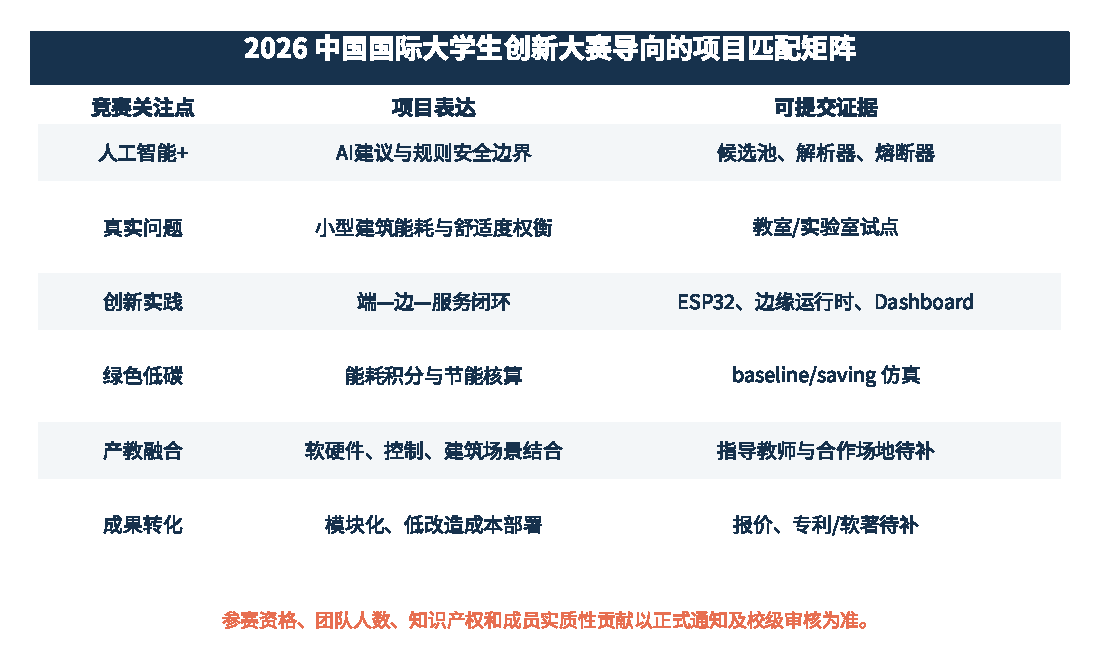
\includegraphics[width=0.93\linewidth]{figures/competition_match.pdf}\caption{项目特征与 2026 中国国际大学生创新大赛关注点的匹配矩阵。}\label{fig:match_manual}\end{figure}
\begin{table}[htbp]\centering\small\caption{作品申报的主张、证据与边界}\begin{tabularx}{\linewidth}{>{\bfseries}p{0.22\linewidth}X p{0.25\linewidth}}\toprule 主张 & 当前证据 & 申报时的边界\\\midrule
人工智能+ & AI 候选池、结构化解析、规则融合与熔断回退 & 不表述为 AI 直接控制物理设备\\
绿色低碳 & 能耗积分公式、baseline/saving 数字孪生对照 & 仿真结果不等于真实建筑节能率\\
创新实践 & ESP32-S3、边缘运行时、API、Dashboard 闭环 & 真实硬件长时运行记录待补\\
成果转化 & 模块化、边缘优先、低改造部署思路 & 成本、客户和合作场地证据待补\\\bottomrule\end{tabularx}\end{table}

\section{用户、痛点与应用场景}
小型建筑空间通常缺少大型楼宇管理系统的预算和运维能力，但仍然面对空调、照明、空气质量和设备安全之间的协同问题。项目将用户分为三类：一是需要低成本试点的学校和实验室管理者；二是需要降低运维复杂度的办公室和小型商业空间；三是需要保留原有设备、逐步接入数字化管理的既有建筑运维人员。项目原始说明材料还提出了低改造成本、模块化部署和无需大规模改线等产品化方向，正式提交时应补充访谈对象、场地面积、设备清单和试点授权。
\begin{figure}[htbp]\centering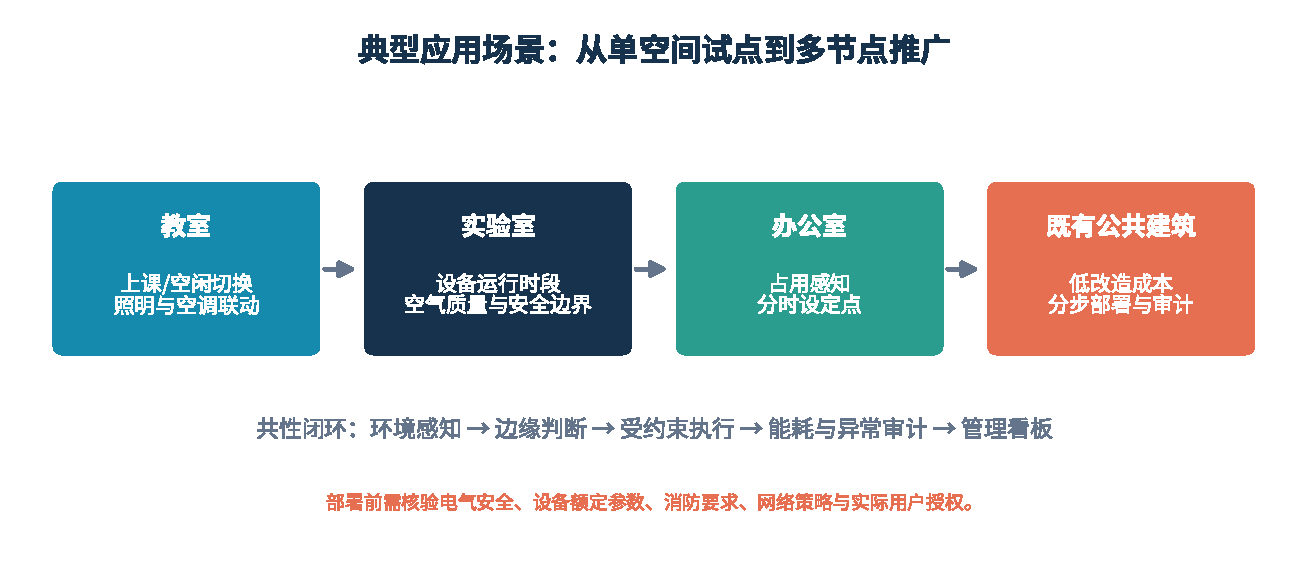
\includegraphics[width=0.96\linewidth]{figures/application_scenarios.pdf}\caption{典型应用场景与共性数据闭环。}\label{fig:scenes_manual}\end{figure}
\begin{table}[htbp]\centering\small\caption{用户痛点与产品回应}\begin{tabularx}{\linewidth}{>{\bfseries}p{0.24\linewidth}X X}\toprule 用户痛点 & 产品回应 & 待补验证材料\\\midrule
设备孤岛 & 串口 JSON、可选 MQTT、多模块适配 & \placeholder{设备型号、协议回放记录}\\
只看环境不看能耗 & 功率采集、JSONL 记录、时间窗口查询 & \placeholder{功率计型号、校准证书}\\
节能后舒适度不稳定 & 滞回、分时设定点、最小启停时间 & \placeholder{舒适度定义、用户评价}\\
AI 建议不可控 & 候选命令、白名单、范围、限频、熔断 & \placeholder{故障注入与审计样例}\\
系统坏了难定位 & stale 检测、I2C 恢复、设备复位、事件记录 & \placeholder{恢复时间与异常日志}\\\bottomrule\end{tabularx}\end{table}

\section{方案对比与产品定义}
传统定时控制成本低但缺少环境反馈；纯云端 AI 便于集中分析却依赖网络；纯本地规则可靠但难以吸收复杂建议。EcoSentinel 的产品定位不是替代所有楼宇自动化系统，而是为小型空间提供一个可以从单节点试点开始、逐步扩展到多节点的边缘优先模块。
\begin{figure}[htbp]\centering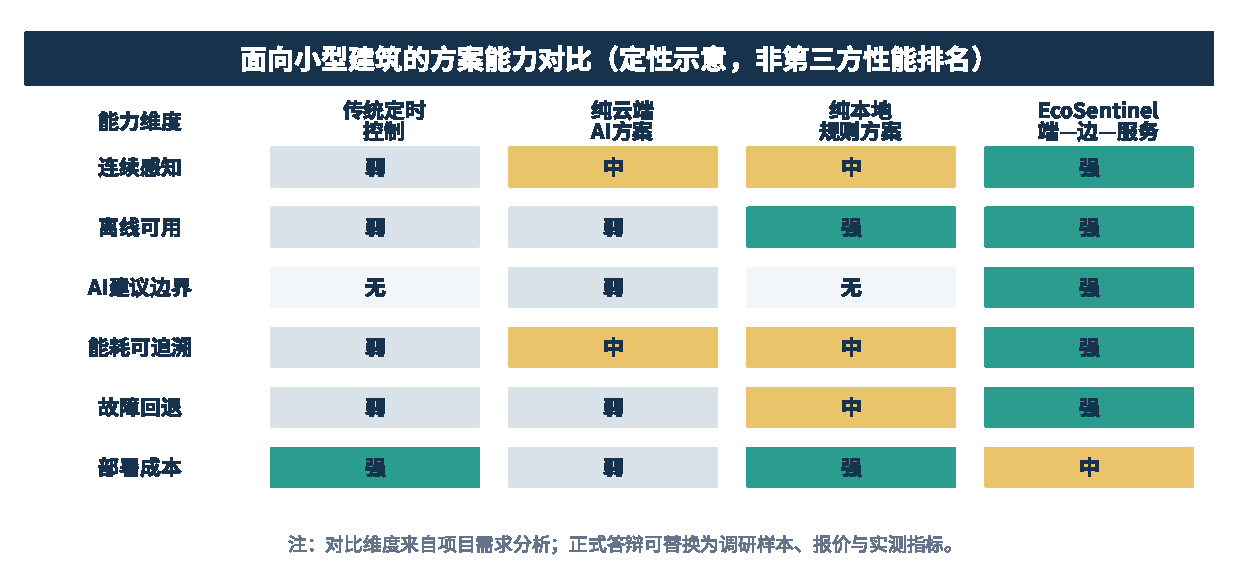
\includegraphics[width=0.96\linewidth]{figures/solution_comparison.pdf}\caption{面向小型建筑的方案能力定性对比；正式版本可替换为调研与实测数据。}\label{fig:comparison_manual}\end{figure}
\begin{table}[htbp]\centering\small\caption{产品功能清单与交付形态}\begin{tabularx}{\linewidth}{>{\bfseries}p{0.22\linewidth}X p{0.25\linewidth}}\toprule 功能模块 & 主要功能 & 交付形态\\\midrule
感知节点 & 温湿度、光照、空气质量、人体与功率信息采集 & ESP32-S3 固件与接线清单\\
边缘控制 & 规则控制、AI 建议融合、离线保护、自愈 & Python 运行时与 YAML 配置\\
数据服务 & JSONL 记录、坏行统计、时间窗口 API、schema 校验 & FastAPI 服务\\
可视化 & 遥测、能耗、异常、实验结果展示 & React/Streamlit Dashboard\\
实验与审计 & 参数、seed、配置哈希、动作和失败原因记录 & 实验清单与可复现包\\\bottomrule\end{tabularx}\end{table}

\section{行业与政策环境}
国际能源署将建筑数字化优化视为提升运行效率的重要路径\cite{iea_efficiency_2025}；我国建筑领域节能降碳工作方案强调建筑运行节能管理、能耗统计核算以及数字化智能化运行管理平台建设\cite{china_building_efficiency_2024}。近年的 BEMS、物联网和人工智能综述也将传感感知、HVAC 优化、占用驱动控制和故障检测视为相互关联的技术方向\cite{bems_iot_ai_2025,iot_smart_buildings_2024}。这些资料支持项目的行业背景与技术方向判断，但不直接证明本项目的节能率；本项目的性能结论仍必须来自自己的可复现实验。

\section{控制策略、节能机理与经济性边界}

\begin{figure}[htbp]\centering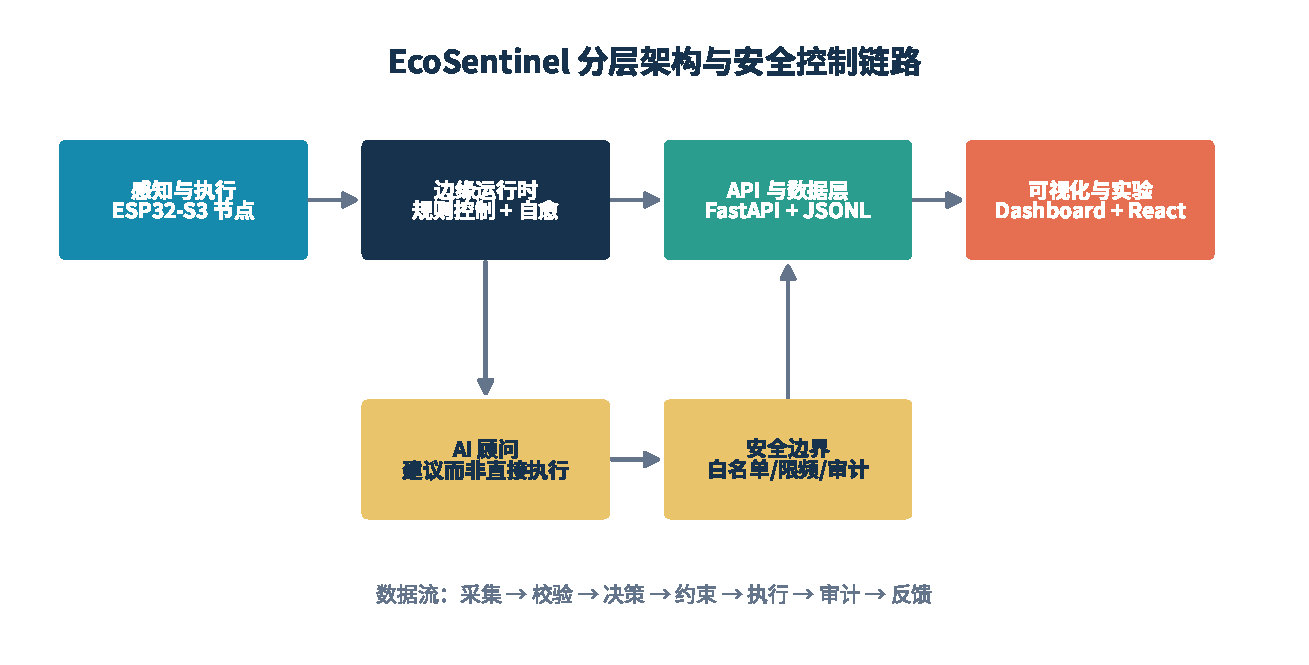
\includegraphics[width=0.97\linewidth]{figures/architecture.pdf}\caption{系统总体架构。}\label{fig:arch2}\end{figure}
系统采用端—边—服务—可视化的分层结构。端侧负责实时采集和执行；边缘侧负责协议解析、规则控制、AI 建议融合、故障恢复和本地记录；服务侧负责只读监控 API、时间窗口查询、坏行统计和响应 schema；可视化侧负责展示遥测、能耗、韧性状态和实验结果。MQTT 可作为可选的发布/订阅通道，其轻量、解耦的特性适合物联网场景\cite{mqtt5}。

\subsection{关键数据链路}
一条完整数据链路为：传感器采样—时间戳封装—JSONL 记录—仓储读取—服务聚合—API schema 校验—Dashboard 展示。仓储层作为 JSONL 的唯一读取入口，显式统计损坏记录，按真实时间窗口过滤，而不是简单按行数截取。这样可以避免日志局部损坏或采样频率变化导致监控结果失真。

\subsection{控制与安全链路}
控制链路为“安全模式—设备离线保护—本地规则—AI 建议融合—动作去抖—最小间隔—执行器发送—结果审计”。AI 顾问不能直接调用串口或绕过命令编译器。可执行命令需要经过语法、范围、数量、权限和限频检查；当 AI 超时、格式错误、连续失败或熔断时，系统回退到本地策略或无动作状态。
\section{硬件与软件实现}
\subsection{ESP32-S3 感知执行节点}
ESP32-S3 作为节点主控，具有双核 LX7、2.4 GHz Wi-Fi、Bluetooth LE，以及 UART、I2C、SPI、ADC 等接口资源\cite{esp32s3}。固件从原单文件 sketch 拆分为 \texttt{config.h}、\texttt{types.h}、\texttt{state.h}、\texttt{actuators.h}、\texttt{sensors.h}、\texttt{protocol.h}、\texttt{display.h} 和 \texttt{mqtt.h}，主 sketch 仅保留 \texttt{setup()} 与 \texttt{loop()}。模块采用 `\#pragma once` 和 static 链接，以保持单翻译单元语义；串口协议字段保持兼容，并在 \texttt{GET\_STATE} 中加入 \texttt{protocol\_version}。

\begin{table}[htbp]\centering\caption{硬件模块与验证状态}\begin{tabularx}{\linewidth}{>{\bfseries}p{0.24\linewidth}X p{0.18\linewidth}}\toprule 模块 & 作用 & 状态\\\midrule 环境传感器 & 温湿度、光照、空气质量 & \placeholder{型号与实测状态}\\ 电能计量 & 功率、电流、电压与累计能耗 & \placeholder{计量芯片/功率计}\\ 执行器 & 继电器、蜂鸣器、窗帘/步进机构 & \placeholder{设备清单}\\ 通信 & 串口 JSON；可选 MQTT & 软件完成，实机待验\\ 显示交互 & TFT 状态屏与按钮 & \placeholder{屏幕型号与照片}\\\bottomrule\end{tabularx}\end{table}

\subsection{软件模块化}
软件侧以领域模型和服务边界替代单文件堆叠。核心目录包括 \texttt{energy\_system/core}、\texttt{energy\_system/application}、\texttt{energy\_system/ai}、\texttt{energy\_system/resilience}、\texttt{energy\_system/api}、\texttt{energy\_system/persistence}、\texttt{energy\_system/power} 和 \texttt{energy\_system/experiments}。FastAPI 采用应用工厂和 Pydantic schema，可自动生成 OpenAPI 相关文档\cite{fastapi}；旧入口仍保留，以降低迁移风险。
\section{控制策略与数学模型}
\subsection{温度控制}
系统采用带滞回的本地控制策略，避免执行器在阈值附近频繁启停。控制器可以写作：
\begin{equation}\label{eq:control}
 u_t=\begin{cases}1,&T_t>T_{\mathrm{set}}+\delta,\\0,&T_t<T_{\mathrm{set}}-\delta,\\u_{t-1},&\text{otherwise},\end{cases}
\end{equation}
其中，\(T_{\mathrm{set}}\) 为设定温度，\(\delta\) 为滞回半宽，\(u_t\) 为设备状态。设备还应满足最小运行时间和最小停止时间约束，具体参数以\placeholder{真实设备参数}为准。

\subsection{能耗核算}
功率积分采用：
\begin{equation}\label{eq:power}E=\frac{1}{3.6\times 10^6}\sum_{i=1}^{n}P_i\Delta t_i.
\end{equation}
节电率为：
\begin{equation}\label{eq:saving}R=\frac{E_{\rm baseline}-E_{\rm saving}}{E_{\rm baseline}}\times100\% .
\end{equation}
若需要碳排放估计，可使用：
\begin{equation}\label{eq:carbon}C=E\times f_{\rm grid},
\end{equation}
其中电网排放因子 \(f_{\rm grid}\) 必须注明来源、地区和版本，不能将占位参数表述为实测结论。
\section{实验设计与结果}
\subsection{数字孪生基线}
当前基线实验采用 3 天时长、300 秒步长、随机种子 42，比较 baseline 与 saving 两种模式。实验输出同时记录模型参数、采样周期、配置哈希和实验清单，从而支持重新运行和结果追溯。可复现性原则包括记录随机种子、代码版本、参数和环境信息\cite{reproducibility}。
\begin{table}[htbp]\centering\caption{当前数字孪生结果；真实实测结果请另行标注}\begin{tabular}{lrrr}\toprule 指标 & baseline & saving & 备注\\\midrule 累计能耗 / kWh & 81.48 & 57.18 & 仿真\\ 节省电量 / kWh & \textemdash & 24.30 & 仿真差值\\ 节电率 / \% & \textemdash & 29.8 & 仿真\\ 平均舒适度 / \% & 82.1 & 82.1 & 仿真\\\bottomrule\end{tabular}\end{table}
\begin{figure}[htbp]\centering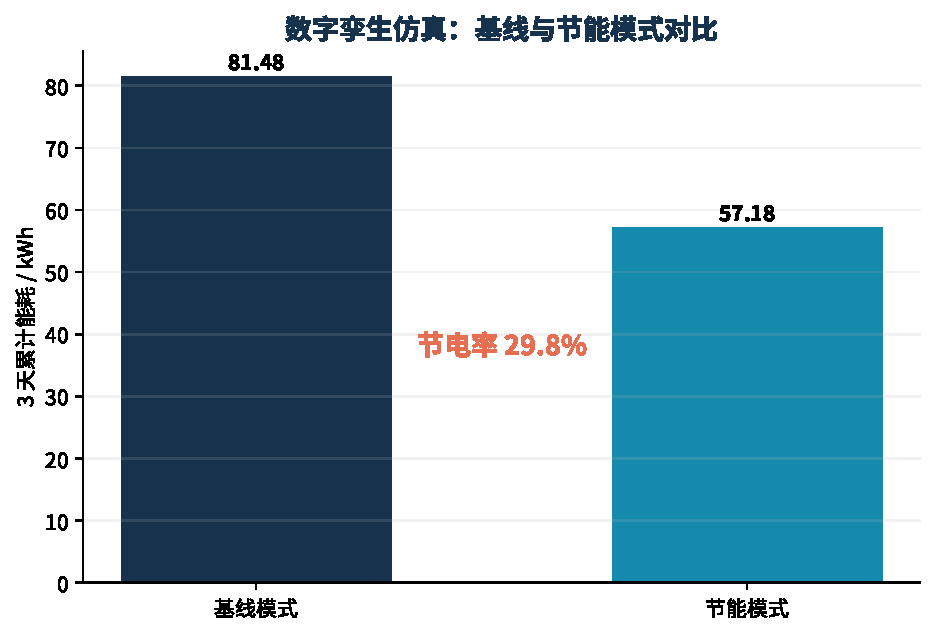
\includegraphics[width=0.70\linewidth]{figures/energy_comparison.pdf}\caption{数字孪生能耗对比。}\end{figure}
\begin{figure}[htbp]\centering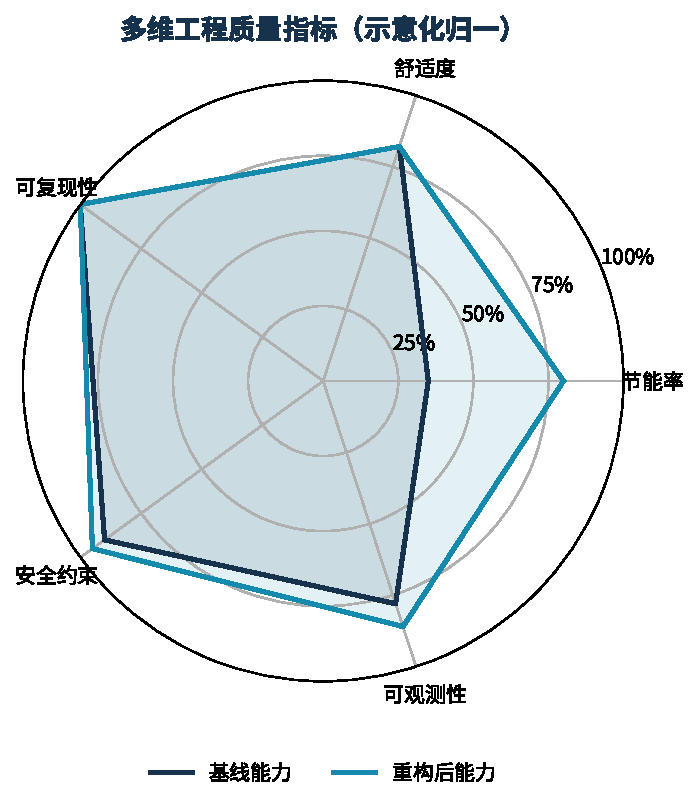
\includegraphics[width=0.72\linewidth]{figures/quality_radar.pdf}\caption{多维工程质量指标的归一化示意；正式提交时应替换为有明确定义和数据来源的指标图。}\end{figure}

\subsection{真实平台实验模板}
真实实验建议采用交叉对照或分时段对照设计。至少记录实验空间、设备额定功率、室外环境、初始温度、人员数量、控制模式、采样周期和异常事件。舒适度评价应明确采用何种定义；如引用热舒适标准，应说明标准版本和适用范围。ASHRAE Standard 55 以温度、辐射、湿度、风速以及活动和衣着等因素讨论人体热环境\cite{ashrae55}，本项目当前的“舒适度百分比”是仿真指标，不能直接等同于标准符合率。
\begin{figure}[htbp]\centering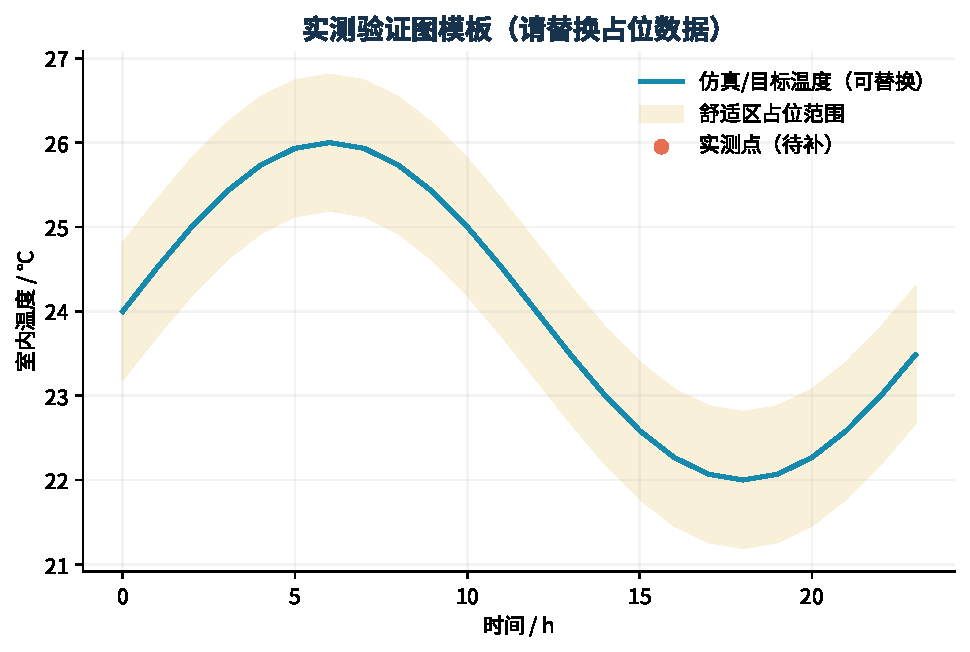
\includegraphics[width=0.75\linewidth]{figures/field_test_template.pdf}\caption{真实平台温度与舒适区图模板；实测点目前为占位符。}\end{figure}
\begin{table}[htbp]\centering\caption{建议补充的真实硬件实验记录}\begin{tabularx}{\linewidth}{>{\bfseries}p{0.25\linewidth}X}\toprule 字段 & 记录内容\\\midrule 实验编号 & \placeholder{EXP-YYYYMMDD-01}\\ 场地与面积 & \placeholder{房间用途、面积、朝向}\\ 设备与量程 & \placeholder{空调、继电器、功率计、传感器型号}\\ 时段与天气 & \placeholder{开始/结束时间、室外温湿度}\\ baseline 结果 & \placeholder{kWh、温度均值、舒适度、异常数}\\ saving 结果 & \placeholder{kWh、温度均值、舒适度、异常数}\\ 统计方法 & \placeholder{均值、标准差、置信区间、效应量}\\\bottomrule\end{tabularx}\end{table}
\section{测试、工程质量与安全审计}
当前软件工程验收包括 Python 148 项测试、compileall、确定性仿真 smoke test、React lint/typecheck/build，以及 GitHub Actions 中的 gitleaks 扫描。CI 的三个 job 均已通过。固件实际编译、串口回放、Wi-Fi/MQTT 连接和真实硬件 smoke test 仍需在配置 Arduino IDE 或 PlatformIO 的环境中完成。

\begin{figure}[htbp]\centering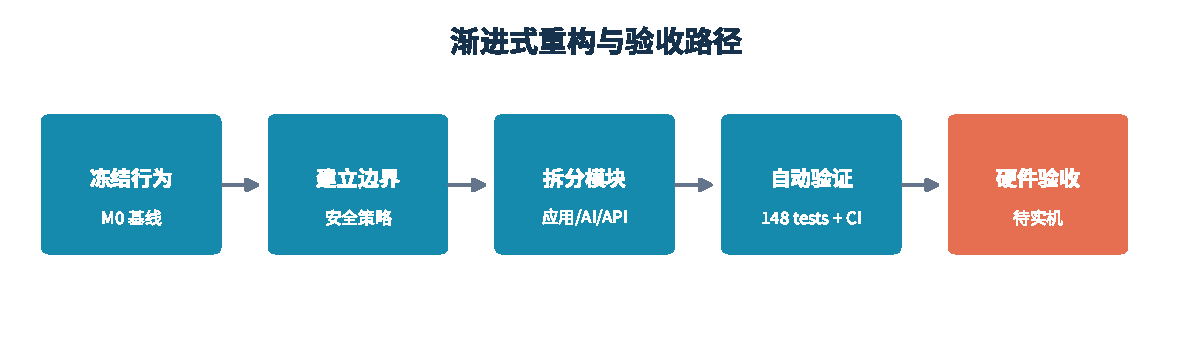
\includegraphics[width=0.97\linewidth]{figures/validation_pipeline.pdf}\caption{软件验收和硬件验收的分界。}\end{figure}
\begin{table}[htbp]\centering\caption{验收状态矩阵}\begin{tabularx}{\linewidth}{>{\bfseries}p{0.32\linewidth}X p{0.18\linewidth}}\toprule 验收项 & 证据 & 状态\\\midrule P0--P11 软件重构 & 分阶段提交、模块结构、兼容入口 & 已完成\\ Python 测试与仿真 & 148 passed；固定 seed 结果一致 & 已验证\\ 前端质量门禁 & lint/typecheck/build 与云端 CI & 已验证\\ 密钥扫描 & gitleaks job success & 已验证\\ ESP32 编译 & 需 Arduino/PlatformIO + 开发板 & 待实机\\ 串口/Wi-Fi/MQTT & 需真实节点和网络环境 & 待实机\\\bottomrule\end{tabularx}\end{table}
\section{创新点与应用价值}
本作品的创新点并不只在于“加入 AI”，而在于把 AI 放入一个有边界的工程闭环中。其一，采用“AI 建议、规则决策、安全执行”的分权结构，降低不可解释动作风险。其二，采用边缘优先的控制方式，使基本能力不依赖云端可用性。其三，将损坏日志统计、实验清单、配置哈希和确定性仿真纳入系统，使节能效果可以被追溯。其四，使用渐进式代码重构将硬件、应用、API、AI 和实验模块分离，便于后续扩展多房间、多设备或需求响应场景。

系统适用于\placeholder{学校实验室、办公室、教室、展厅或其他应用场景}。部署前需要重新确认电气安全、继电器额定参数、网络安全策略和当地用能管理要求。作品不应被表述为已经完成大规模商业部署，也不应把仿真结果替代为实测数据。
\section{不足与后续计划}
当前不足主要包括：真实硬件实验样本量仍需扩大；传感器校准和电表误差需要量化；舒适度指标需要与标准或用户评价建立更清晰的对应关系；仿真报告中的时间元数据仍可通过注入时钟实现更严格的字节级快照；前端 bundle 分包和 Browserslist 更新属于后续 P2 优化。

后续计划分为三个阶段。第一阶段完成固件编译、串口回放和硬件 smoke test；第二阶段开展不少于\placeholder{N}组的 baseline/saving 交叉实验；第三阶段建立多节点协同、异常预测和需求响应实验，并报告均值、方差、置信区间和可复现实验包。
\section{结论}
EcoSentinel 构建了一个从环境感知到节能控制、从 AI 建议到安全审计、从数据记录到实验复现的完整原型。软件侧 P0--P11 重构、自动化测试和云端质量门禁已经完成；硬件侧仍需真实环境完成最终编译与运行验证。项目的核心价值在于：把节能目标、舒适度约束、AI 能力和工程可验证性统一到一条可追踪链路中。
\section*{材料替换说明}
文中所有橙色“待补”字段均可直接替换。正式提交前请检查：项目名称与团队信息、图片版权与来源、仿真/实测标签、实验日期、硬件型号、统计口径、引用文献版本和竞赛格式要求。
\printbibliography
\end{document}
